\documentclass[1p]{elsarticle_modified}
%\bibliographystyle{elsarticle-num}

%\usepackage[colorlinks]{hyperref}
%\usepackage{abbrmath_seonhwa} %\Abb, \Ascr, \Acal ,\Abf, \Afrak
\usepackage{amsfonts}
\usepackage{amssymb}
\usepackage{amsmath}
\usepackage{amsthm}
\usepackage{scalefnt}
\usepackage{amsbsy}
\usepackage{kotex}
\usepackage{caption}
\usepackage{subfig}
\usepackage{color}
\usepackage{graphicx}
\usepackage{xcolor} %% white, black, red, green, blue, cyan, magenta, yellow
\usepackage{float}
\usepackage{setspace}
\usepackage{hyperref}

\usepackage{tikz}
\usetikzlibrary{arrows}

\usepackage{multirow}
\usepackage{array} % fixed length table
\usepackage{hhline}

%%%%%%%%%%%%%%%%%%%%%
\makeatletter
\renewcommand*\env@matrix[1][\arraystretch]{%
	\edef\arraystretch{#1}%
	\hskip -\arraycolsep
	\let\@ifnextchar\new@ifnextchar
	\array{*\c@MaxMatrixCols c}}
\makeatother %https://tex.stackexchange.com/questions/14071/how-can-i-increase-the-line-spacing-in-a-matrix
%%%%%%%%%%%%%%%

\usepackage[normalem]{ulem}

\newcommand{\msout}[1]{\ifmmode\text{\sout{\ensuremath{#1}}}\else\sout{#1}\fi}
%SOURCE: \msout is \stkout macro in https://tex.stackexchange.com/questions/20609/strikeout-in-math-mode

\newcommand{\cancel}[1]{
	\ifmmode
	{\color{red}\msout{#1}}
	\else
	{\color{red}\sout{#1}}
	\fi
}

\newcommand{\add}[1]{
	{\color{blue}\uwave{#1}}
}

\newcommand{\replace}[2]{
	\ifmmode
	{\color{red}\msout{#1}}{\color{blue}\uwave{#2}}
	\else
	{\color{red}\sout{#1}}{\color{blue}\uwave{#2}}
	\fi
}

\newcommand{\Sol}{\mathcal{S}} %segment
\newcommand{\D}{D} %diagram
\newcommand{\A}{\mathcal{A}} %arc


%%%%%%%%%%%%%%%%%%%%%%%%%%%%%5 test

\def\sl{\operatorname{\textup{SL}}(2,\Cbb)}
\def\psl{\operatorname{\textup{PSL}}(2,\Cbb)}
\def\quan{\mkern 1mu \triangleright \mkern 1mu}

\theoremstyle{definition}
\newtheorem{thm}{Theorem}[section]
\newtheorem{prop}[thm]{Proposition}
\newtheorem{lem}[thm]{Lemma}
\newtheorem{ques}[thm]{Question}
\newtheorem{cor}[thm]{Corollary}
\newtheorem{defn}[thm]{Definition}
\newtheorem{exam}[thm]{Example}
\newtheorem{rmk}[thm]{Remark}
\newtheorem{alg}[thm]{Algorithm}

\newcommand{\I}{\sqrt{-1}}
\begin{document}

%\begin{frontmatter}
%
%\title{Boundary parabolic representations of knots up to 8 crossings}
%
%%% Group authors per affiliation:
%\author{Yunhi Cho} 
%\address{Department of Mathematics, University of Seoul, Seoul, Korea}
%\ead{yhcho@uos.ac.kr}
%
%
%\author{Seonhwa Kim} %\fnref{s_kim}}
%\address{Center for Geometry and Physics, Institute for Basic Science, Pohang, 37673, Korea}
%\ead{ryeona17@ibs.re.kr}
%
%\author{Hyuk Kim}
%\address{Department of Mathematical Sciences, Seoul National University, Seoul 08826, Korea}
%\ead{hyukkim@snu.ac.kr}
%
%\author{Seokbeom Yoon}
%\address{Department of Mathematical Sciences, Seoul National University, Seoul, 08826,  Korea}
%\ead{sbyoon15@snu.ac.kr}
%
%\begin{abstract}
%We find all boundary parabolic representation of knots up to 8 crossings.
%
%\end{abstract}
%\begin{keyword}
%    \MSC[2010] 57M25 
%\end{keyword}
%
%\end{frontmatter}

%\linenumbers
%\tableofcontents
%
\newcommand\colored[1]{\textcolor{white}{\rule[-0.35ex]{0.8em}{1.4ex}}\kern-0.8em\color{red} #1}%
%\newcommand\colored[1]{\textcolor{white}{ #1}\kern-2.17ex	\textcolor{white}{ #1}\kern-1.81ex	\textcolor{white}{ #1}\kern-2.15ex\color{red}#1	}

{\Large $\underline{12a_{0013}~(K12a_{0013})}$}

\setlength{\tabcolsep}{10pt}
\renewcommand{\arraystretch}{1.6}
\vspace{1cm}\begin{tabular}{m{100pt}>{\centering\arraybackslash}m{274pt}}
\multirow{5}{120pt}{
	\centering
	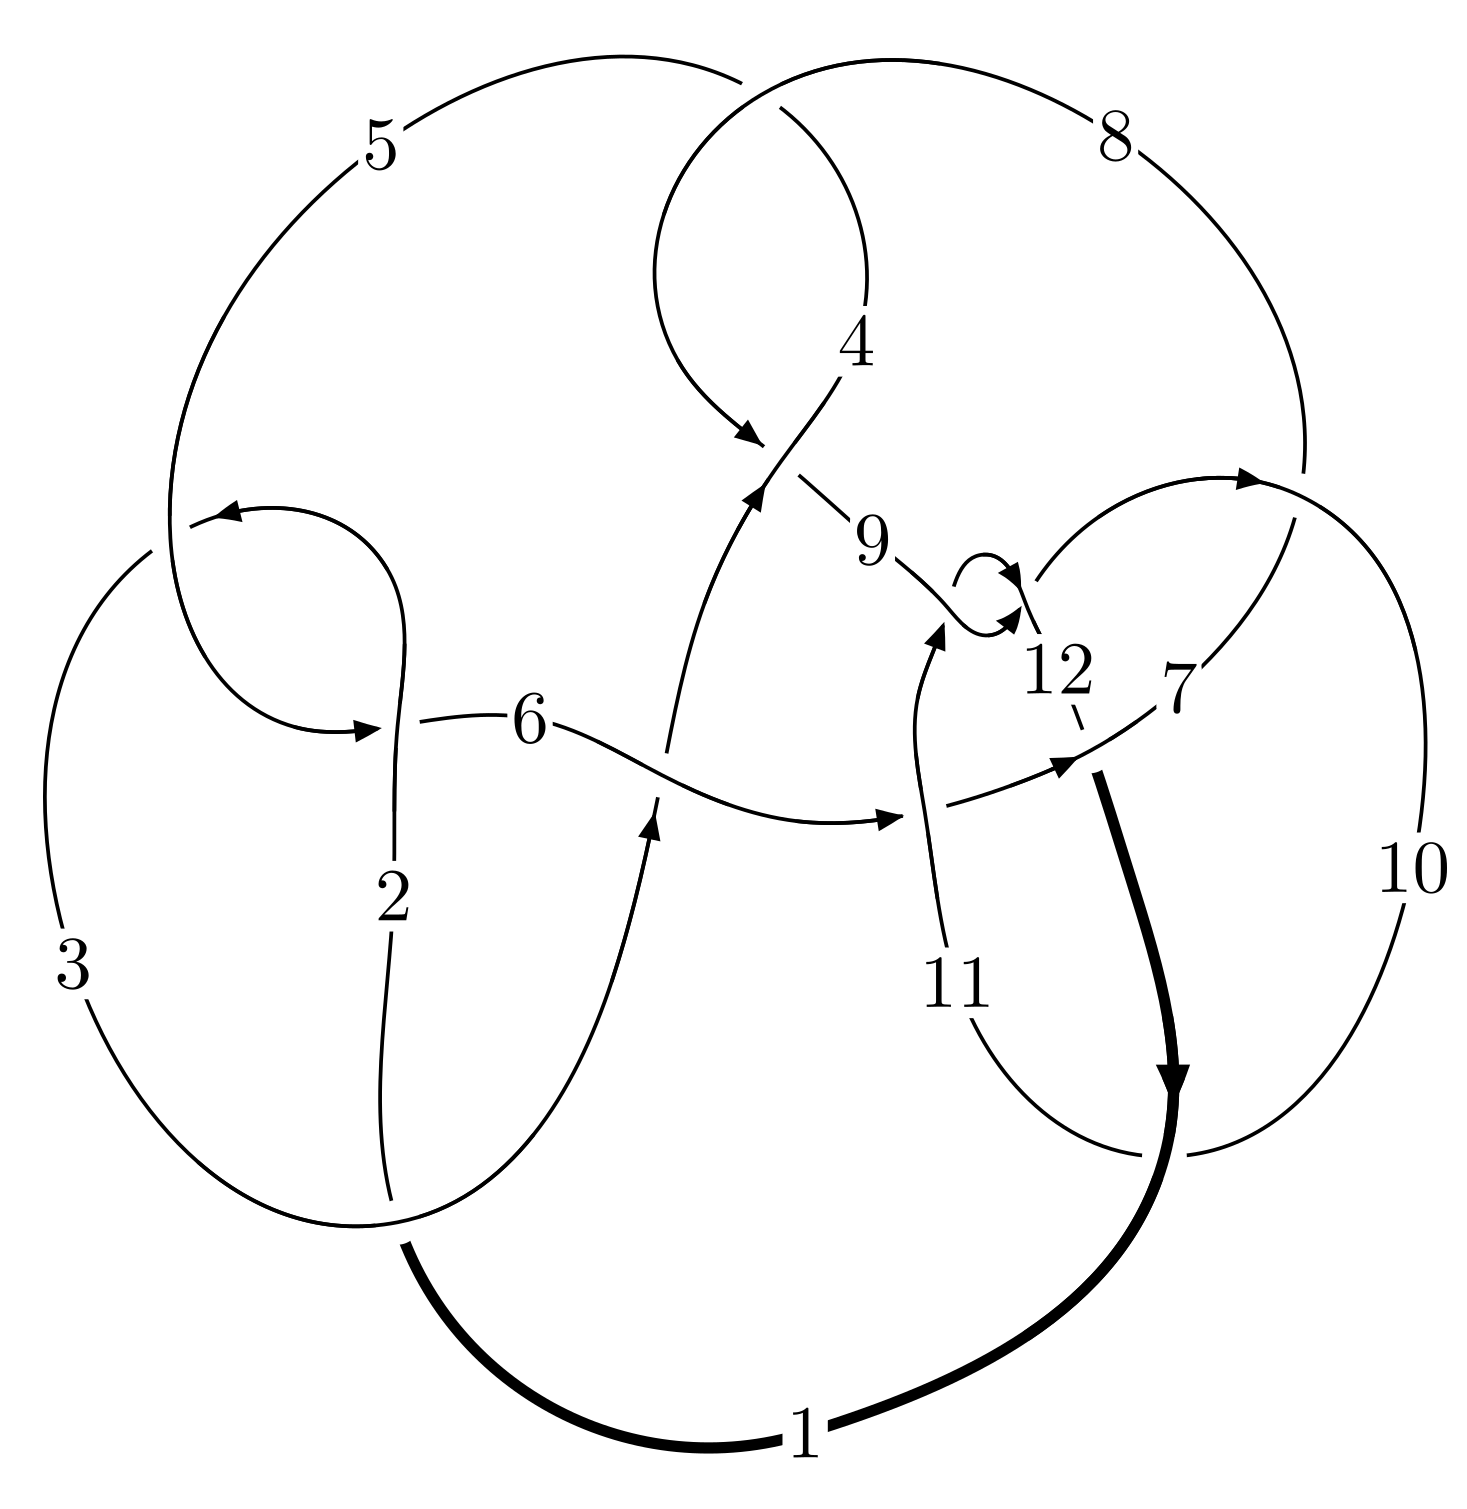
\includegraphics[width=112pt]{../../../GIT/diagram.site/Diagrams/png/814_12a_0013.png}\\
\ \ \ A knot diagram\footnotemark}&
\allowdisplaybreaks
\textbf{Linearized knot diagam} \\
\cline{2-2}
 &
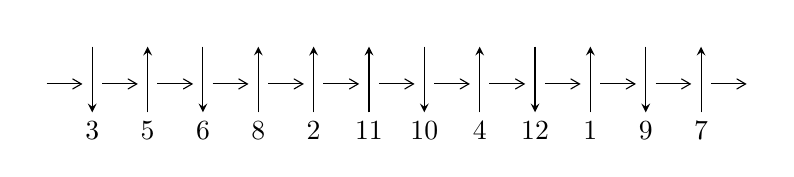
\begin{tikzpicture}[x=20pt, y=17pt]
	% nodes
	\node (C0) at (0, 0) {};
	\node (C1) at (1, 0) {};
	\node (C1U) at (1, +1) {};
	\node (C1D) at (1, -1) {3};

	\node (C2) at (2, 0) {};
	\node (C2U) at (2, +1) {};
	\node (C2D) at (2, -1) {5};

	\node (C3) at (3, 0) {};
	\node (C3U) at (3, +1) {};
	\node (C3D) at (3, -1) {6};

	\node (C4) at (4, 0) {};
	\node (C4U) at (4, +1) {};
	\node (C4D) at (4, -1) {8};

	\node (C5) at (5, 0) {};
	\node (C5U) at (5, +1) {};
	\node (C5D) at (5, -1) {2};

	\node (C6) at (6, 0) {};
	\node (C6U) at (6, +1) {};
	\node (C6D) at (6, -1) {11};

	\node (C7) at (7, 0) {};
	\node (C7U) at (7, +1) {};
	\node (C7D) at (7, -1) {10};

	\node (C8) at (8, 0) {};
	\node (C8U) at (8, +1) {};
	\node (C8D) at (8, -1) {4};

	\node (C9) at (9, 0) {};
	\node (C9U) at (9, +1) {};
	\node (C9D) at (9, -1) {12};

	\node (C10) at (10, 0) {};
	\node (C10U) at (10, +1) {};
	\node (C10D) at (10, -1) {1};

	\node (C11) at (11, 0) {};
	\node (C11U) at (11, +1) {};
	\node (C11D) at (11, -1) {9};

	\node (C12) at (12, 0) {};
	\node (C12U) at (12, +1) {};
	\node (C12D) at (12, -1) {7};
	\node (C13) at (13, 0) {};

	% arrows
	\draw[->,>={angle 60}]
	(C0) edge (C1) (C1) edge (C2) (C2) edge (C3) (C3) edge (C4) (C4) edge (C5) (C5) edge (C6) (C6) edge (C7) (C7) edge (C8) (C8) edge (C9) (C9) edge (C10) (C10) edge (C11) (C11) edge (C12) (C12) edge (C13) ;	\draw[->,>=stealth]
	(C1U) edge (C1D) (C2D) edge (C2U) (C3U) edge (C3D) (C4D) edge (C4U) (C5D) edge (C5U) (C6D) edge (C6U) (C7U) edge (C7D) (C8D) edge (C8U) (C9U) edge (C9D) (C10D) edge (C10U) (C11U) edge (C11D) (C12D) edge (C12U) ;
	\end{tikzpicture} \\
\hhline{~~} \\& 
\textbf{Solving Sequence} \\ \cline{2-2} 
 &
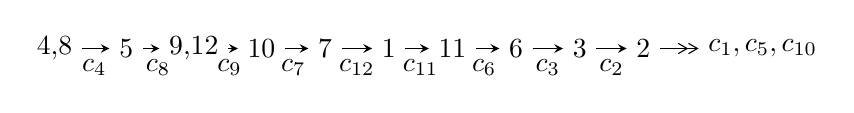
\begin{tikzpicture}[x=23pt, y=7pt]
	% node
	\node (A0) at (-1/8, 0) {4,8};
	\node (A1) at (1, 0) {5};
	\node (A2) at (33/16, 0) {9,12};
	\node (A3) at (25/8, 0) {10};
	\node (A4) at (33/8, 0) {7};
	\node (A5) at (41/8, 0) {1};
	\node (A6) at (49/8, 0) {11};
	\node (A7) at (57/8, 0) {6};
	\node (A8) at (65/8, 0) {3};
	\node (A9) at (73/8, 0) {2};
	\node (C1) at (1/2, -1) {$c_{4}$};
	\node (C2) at (3/2, -1) {$c_{8}$};
	\node (C3) at (21/8, -1) {$c_{9}$};
	\node (C4) at (29/8, -1) {$c_{7}$};
	\node (C5) at (37/8, -1) {$c_{12}$};
	\node (C6) at (45/8, -1) {$c_{11}$};
	\node (C7) at (53/8, -1) {$c_{6}$};
	\node (C8) at (61/8, -1) {$c_{3}$};
	\node (C9) at (69/8, -1) {$c_{2}$};
	\node (A10) at (11, 0) {$c_{1},c_{5},c_{10}$};

	% edge
	\draw[->,>=stealth]	
	(A0) edge (A1) (A1) edge (A2) (A2) edge (A3) (A3) edge (A4) (A4) edge (A5) (A5) edge (A6) (A6) edge (A7) (A7) edge (A8) (A8) edge (A9) ;
	\draw[->>,>={angle 60}]	
	(A9) edge (A10);
\end{tikzpicture} \\ 

\end{tabular} \\

\footnotetext{
The image of knot diagram is generated by the software ``\textbf{Draw programme}" developed by Andrew Bartholomew(\url{http://www.layer8.co.uk/maths/draw/index.htm\#Running-draw}), where we modified some parts for our purpose(\url{https://github.com/CATsTAILs/LinksPainter}).
}\phantom \\ \newline 
\centering \textbf{Ideals for irreducible components\footnotemark of $X_{\text{par}}$} 
 
\begin{align*}
I^u_{1}&=\langle 
-1.02573\times10^{605} u^{137}-5.51686\times10^{604} u^{136}+\cdots+1.68194\times10^{607} b-1.50040\times10^{609},\\
\phantom{I^u_{1}}&\phantom{= \langle  }-1.26961\times10^{605} u^{137}+7.22190\times10^{603} u^{136}+\cdots+3.36387\times10^{607} a-1.61972\times10^{609},\\
\phantom{I^u_{1}}&\phantom{= \langle  }u^{138}- u^{137}+\cdots+20480 u+4096\rangle \\
\\
I^v_{1}&=\langle 
a,\;1003453 v^{11}+865361 v^{10}+\cdots+707733 b+3119402,\\
\phantom{I^v_{1}}&\phantom{= \langle  }v^{12}+v^{11}-4 v^{10}+5 v^9+19 v^8-9 v^7-31 v^6-29 v^5+31 v^4+18 v^3+3 v^2+3 v+1\rangle \\
\end{align*}
\raggedright * 2 irreducible components of $\dim_{\mathbb{C}}=0$, with total 150 representations.\\
\footnotetext{All coefficients of polynomials are rational numbers. But the coefficients are sometimes approximated in decimal forms when there is not enough margin.}
\newpage
\renewcommand{\arraystretch}{1}
\centering \section*{I. $I^u_{1}= \langle -1.03\times10^{605} u^{137}-5.52\times10^{604} u^{136}+\cdots+1.68\times10^{607} b-1.50\times10^{609},\;-1.27\times10^{605} u^{137}+7.22\times10^{603} u^{136}+\cdots+3.36\times10^{607} a-1.62\times10^{609},\;u^{138}- u^{137}+\cdots+20480 u+4096 \rangle$}
\flushleft \textbf{(i) Arc colorings}\\
\begin{tabular}{m{7pt} m{180pt} m{7pt} m{180pt} }
\flushright $a_{4}=$&$\begin{pmatrix}1\\0\end{pmatrix}$ \\
\flushright $a_{8}=$&$\begin{pmatrix}0\\u\end{pmatrix}$ \\
\flushright $a_{5}=$&$\begin{pmatrix}1\\- u^2\end{pmatrix}$ \\
\flushright $a_{9}=$&$\begin{pmatrix}u\\u\end{pmatrix}$ \\
\flushright $a_{12}=$&$\begin{pmatrix}0.00377426 u^{137}-0.000214690 u^{136}+\cdots+293.153 u+48.1505\\0.00609849 u^{137}+0.00328006 u^{136}+\cdots+526.701 u+89.2069\end{pmatrix}$ \\
\flushright $a_{10}=$&$\begin{pmatrix}0.00379341 u^{137}-0.000460878 u^{136}+\cdots+240.394 u+41.2322\\-0.000165105 u^{137}+0.00929262 u^{136}+\cdots+481.361 u+91.1423\end{pmatrix}$ \\
\flushright $a_{7}=$&$\begin{pmatrix}-0.00238794 u^{137}+0.00493619 u^{136}+\cdots+123.217 u+26.1622\\-0.00357361 u^{137}+0.00819517 u^{136}+\cdots+291.628 u+68.2308\end{pmatrix}$ \\
\flushright $a_{1}=$&$\begin{pmatrix}0.00439295 u^{137}-0.00147919 u^{136}+\cdots+168.616 u+28.0993\\0.00376122 u^{137}+0.00304781 u^{136}+\cdots+360.623 u+65.1201\end{pmatrix}$ \\
\flushright $a_{11}=$&$\begin{pmatrix}0.00261300 u^{137}-0.00172294 u^{136}+\cdots+164.460 u+24.3159\\0.00493724 u^{137}+0.00177181 u^{136}+\cdots+398.008 u+65.3723\end{pmatrix}$ \\
\flushright $a_{6}=$&$\begin{pmatrix}-0.00223744 u^{137}+0.00437981 u^{136}+\cdots+114.339 u+25.0860\\0.00215551 u^{137}+0.00290062 u^{136}+\cdots+282.955 u+53.1853\end{pmatrix}$ \\
\flushright $a_{3}=$&$\begin{pmatrix}0.00294739 u^{137}+0.000658646 u^{136}+\cdots+125.123 u+20.7746\\0.00255322 u^{137}+0.00251675 u^{136}+\cdots+220.759 u+39.9007\end{pmatrix}$ \\
\flushright $a_{2}=$&$\begin{pmatrix}0.00113636 u^{137}-0.000399544 u^{136}+\cdots-9.71148 u-4.35571\\0.00149437 u^{137}+0.00230841 u^{136}+\cdots+154.579 u+28.1483\end{pmatrix}$\\&\end{tabular}
\flushleft \textbf{(ii) Obstruction class $= -1$}\\~\\
\flushleft \textbf{(iii) Cusp Shapes $= -0.0290540 u^{137}+0.0285193 u^{136}+\cdots-46.2850 u+54.5174$}\\~\\
\newpage\renewcommand{\arraystretch}{1}
\flushleft \textbf{(iv) u-Polynomials at the component}\newline \\
\begin{tabular}{m{50pt}|m{274pt}}
Crossings & \hspace{64pt}u-Polynomials at each crossing \\
\hline $$\begin{aligned}c_{1}\end{aligned}$$&$\begin{aligned}
&u^{138}+67 u^{137}+\cdots+33 u+1
\end{aligned}$\\
\hline $$\begin{aligned}c_{2},c_{5}\end{aligned}$$&$\begin{aligned}
&u^{138}+7 u^{137}+\cdots+9 u+1
\end{aligned}$\\
\hline $$\begin{aligned}c_{3}\end{aligned}$$&$\begin{aligned}
&u^{138}-7 u^{137}+\cdots-98472303 u+13657673
\end{aligned}$\\
\hline $$\begin{aligned}c_{4},c_{8}\end{aligned}$$&$\begin{aligned}
&u^{138}- u^{137}+\cdots+20480 u+4096
\end{aligned}$\\
\hline $$\begin{aligned}c_{6}\end{aligned}$$&$\begin{aligned}
&u^{138}-3 u^{137}+\cdots+206471 u+14069
\end{aligned}$\\
\hline $$\begin{aligned}c_{7}\end{aligned}$$&$\begin{aligned}
&u^{138}-9 u^{137}+\cdots+30021 u-1831
\end{aligned}$\\
\hline $$\begin{aligned}c_{9},c_{11}\end{aligned}$$&$\begin{aligned}
&u^{138}-3 u^{137}+\cdots-23 u+1
\end{aligned}$\\
\hline $$\begin{aligned}c_{10}\end{aligned}$$&$\begin{aligned}
&u^{138}+23 u^{137}+\cdots+3 u+1
\end{aligned}$\\
\hline $$\begin{aligned}c_{12}\end{aligned}$$&$\begin{aligned}
&u^{138}+9 u^{137}+\cdots+3 u+1
\end{aligned}$\\
\hline
\end{tabular}\\~\\
\newpage\renewcommand{\arraystretch}{1}
\flushleft \textbf{(v) Riley Polynomials at the component}\newline \\
\begin{tabular}{m{50pt}|m{274pt}}
Crossings & \hspace{64pt}Riley Polynomials at each crossing \\
\hline $$\begin{aligned}c_{1}\end{aligned}$$&$\begin{aligned}
&y^{138}+15 y^{137}+\cdots-35 y+1
\end{aligned}$\\
\hline $$\begin{aligned}c_{2},c_{5}\end{aligned}$$&$\begin{aligned}
&y^{138}+67 y^{137}+\cdots+33 y+1
\end{aligned}$\\
\hline $$\begin{aligned}c_{3}\end{aligned}$$&$\begin{aligned}
&y^{138}-37 y^{137}+\cdots+2159732187820305 y+186532031774929
\end{aligned}$\\
\hline $$\begin{aligned}c_{4},c_{8}\end{aligned}$$&$\begin{aligned}
&y^{138}+65 y^{137}+\cdots+503316480 y+16777216
\end{aligned}$\\
\hline $$\begin{aligned}c_{6}\end{aligned}$$&$\begin{aligned}
&y^{138}-109 y^{137}+\cdots+23684604833 y+197936761
\end{aligned}$\\
\hline $$\begin{aligned}c_{7}\end{aligned}$$&$\begin{aligned}
&y^{138}-137 y^{137}+\cdots-472810103 y+3352561
\end{aligned}$\\
\hline $$\begin{aligned}c_{9},c_{11}\end{aligned}$$&$\begin{aligned}
&y^{138}-89 y^{137}+\cdots-23 y+1
\end{aligned}$\\
\hline $$\begin{aligned}c_{10}\end{aligned}$$&$\begin{aligned}
&y^{138}-9 y^{137}+\cdots-23 y+1
\end{aligned}$\\
\hline $$\begin{aligned}c_{12}\end{aligned}$$&$\begin{aligned}
&y^{138}+23 y^{137}+\cdots+9 y+1
\end{aligned}$\\
\hline
\end{tabular}\\~\\
\newpage\flushleft \textbf{(vi) Complex Volumes and Cusp Shapes}
$$\begin{array}{c|c|c}  
\text{Solutions to }I^u_{1}& \I (\text{vol} + \sqrt{-1}CS) & \text{Cusp shape}\\
 \hline 
\begin{aligned}
u &= -0.225717 + 0.984869 I \\
a &= \phantom{-}0.579663 + 0.604540 I \\
b &= -0.387131 + 0.194000 I\end{aligned}
 & -2.26109 + 1.21839 I & \phantom{-0.000000 } 0 \\ \hline\begin{aligned}
u &= -0.225717 - 0.984869 I \\
a &= \phantom{-}0.579663 - 0.604540 I \\
b &= -0.387131 - 0.194000 I\end{aligned}
 & -2.26109 - 1.21839 I & \phantom{-0.000000 } 0 \\ \hline\begin{aligned}
u &= \phantom{-}0.968613 + 0.291315 I \\
a &= -1.180740 + 0.387329 I \\
b &= \phantom{-}0.252559 + 0.591464 I\end{aligned}
 & -3.85751 - 5.17156 I & \phantom{-0.000000 } 0 \\ \hline\begin{aligned}
u &= \phantom{-}0.968613 - 0.291315 I \\
a &= -1.180740 - 0.387329 I \\
b &= \phantom{-}0.252559 - 0.591464 I\end{aligned}
 & -3.85751 + 5.17156 I & \phantom{-0.000000 } 0 \\ \hline\begin{aligned}
u &= -0.844113 + 0.492611 I \\
a &= \phantom{-}0.158255 - 0.087896 I \\
b &= -0.269909 + 0.863925 I\end{aligned}
 & \phantom{-}2.70862 + 2.80444 I & \phantom{-0.000000 } 0 \\ \hline\begin{aligned}
u &= -0.844113 - 0.492611 I \\
a &= \phantom{-}0.158255 + 0.087896 I \\
b &= -0.269909 - 0.863925 I\end{aligned}
 & \phantom{-}2.70862 - 2.80444 I & \phantom{-0.000000 } 0 \\ \hline\begin{aligned}
u &= -0.495236 + 0.898497 I \\
a &= \phantom{-}0.019024 - 0.146844 I \\
b &= \phantom{-}0.948882 - 0.570151 I\end{aligned}
 & \phantom{-}2.48949 - 5.71532 I & \phantom{-0.000000 } 0 \\ \hline\begin{aligned}
u &= -0.495236 - 0.898497 I \\
a &= \phantom{-}0.019024 + 0.146844 I \\
b &= \phantom{-}0.948882 + 0.570151 I\end{aligned}
 & \phantom{-}2.48949 + 5.71532 I & \phantom{-0.000000 } 0 \\ \hline\begin{aligned}
u &= \phantom{-}0.407051 + 0.951666 I \\
a &= -1.52335 + 1.26262 I \\
b &= -1.074140 + 0.684833 I\end{aligned}
 & -1.49189 + 2.01388 I & \phantom{-0.000000 } 0 \\ \hline\begin{aligned}
u &= \phantom{-}0.407051 - 0.951666 I \\
a &= -1.52335 - 1.26262 I \\
b &= -1.074140 - 0.684833 I\end{aligned}
 & -1.49189 - 2.01388 I & \phantom{-0.000000 } 0\\
 \hline 
 \end{array}$$\newpage$$\begin{array}{c|c|c}  
\text{Solutions to }I^u_{1}& \I (\text{vol} + \sqrt{-1}CS) & \text{Cusp shape}\\
 \hline 
\begin{aligned}
u &= \phantom{-}0.691921 + 0.666142 I \\
a &= \phantom{-}0.456057 - 0.396135 I \\
b &= \phantom{-}0.126915 + 0.564332 I\end{aligned}
 & \phantom{-}1.63530 + 4.17072 I & \phantom{-0.000000 } 0 \\ \hline\begin{aligned}
u &= \phantom{-}0.691921 - 0.666142 I \\
a &= \phantom{-}0.456057 + 0.396135 I \\
b &= \phantom{-}0.126915 - 0.564332 I\end{aligned}
 & \phantom{-}1.63530 - 4.17072 I & \phantom{-0.000000 } 0 \\ \hline\begin{aligned}
u &= \phantom{-}0.647033 + 0.696244 I \\
a &= \phantom{-}0.422005 + 0.408919 I \\
b &= \phantom{-}0.283663 + 0.509054 I\end{aligned}
 & \phantom{-}1.41425 + 1.45110 I & \phantom{-0.000000 } 0 \\ \hline\begin{aligned}
u &= \phantom{-}0.647033 - 0.696244 I \\
a &= \phantom{-}0.422005 - 0.408919 I \\
b &= \phantom{-}0.283663 - 0.509054 I\end{aligned}
 & \phantom{-}1.41425 - 1.45110 I & \phantom{-0.000000 } 0 \\ \hline\begin{aligned}
u &= \phantom{-}0.362183 + 0.876985 I \\
a &= -0.912633 - 0.186335 I \\
b &= -0.132549 + 0.693970 I\end{aligned}
 & \phantom{-}1.44585 + 2.70079 I & \phantom{-0.000000 } 0 \\ \hline\begin{aligned}
u &= \phantom{-}0.362183 - 0.876985 I \\
a &= -0.912633 + 0.186335 I \\
b &= -0.132549 - 0.693970 I\end{aligned}
 & \phantom{-}1.44585 - 2.70079 I & \phantom{-0.000000 } 0 \\ \hline\begin{aligned}
u &= \phantom{-}0.924692 + 0.109605 I \\
a &= -1.024280 - 0.180693 I \\
b &= \phantom{-}0.441690 - 0.778597 I\end{aligned}
 & -4.26855 - 1.64031 I & \phantom{-0.000000 } 0 \\ \hline\begin{aligned}
u &= \phantom{-}0.924692 - 0.109605 I \\
a &= -1.024280 + 0.180693 I \\
b &= \phantom{-}0.441690 + 0.778597 I\end{aligned}
 & -4.26855 + 1.64031 I & \phantom{-0.000000 } 0 \\ \hline\begin{aligned}
u &= -0.790483 + 0.476530 I \\
a &= -0.438850 + 0.486313 I \\
b &= -0.469636 + 0.639265 I\end{aligned}
 & -0.04648 + 3.17550 I & \phantom{-0.000000 } 0 \\ \hline\begin{aligned}
u &= -0.790483 - 0.476530 I \\
a &= -0.438850 - 0.486313 I \\
b &= -0.469636 - 0.639265 I\end{aligned}
 & -0.04648 - 3.17550 I & \phantom{-0.000000 } 0\\
 \hline 
 \end{array}$$\newpage$$\begin{array}{c|c|c}  
\text{Solutions to }I^u_{1}& \I (\text{vol} + \sqrt{-1}CS) & \text{Cusp shape}\\
 \hline 
\begin{aligned}
u &= \phantom{-}0.883665 + 0.175408 I \\
a &= \phantom{-}0.321753 - 0.009471 I \\
b &= \phantom{-}0.645569 + 0.875733 I\end{aligned}
 & -0.821300 - 0.506241 I & \phantom{-0.000000 } 0 \\ \hline\begin{aligned}
u &= \phantom{-}0.883665 - 0.175408 I \\
a &= \phantom{-}0.321753 + 0.009471 I \\
b &= \phantom{-}0.645569 - 0.875733 I\end{aligned}
 & -0.821300 + 0.506241 I & \phantom{-0.000000 } 0 \\ \hline\begin{aligned}
u &= -0.466251 + 0.764985 I \\
a &= \phantom{-}0.069690 - 0.681203 I \\
b &= \phantom{-}0.033362 + 0.508845 I\end{aligned}
 & \phantom{-}0.18427 - 8.79554 I & \phantom{-0.000000 } 0 \\ \hline\begin{aligned}
u &= -0.466251 - 0.764985 I \\
a &= \phantom{-}0.069690 + 0.681203 I \\
b &= \phantom{-}0.033362 - 0.508845 I\end{aligned}
 & \phantom{-}0.18427 + 8.79554 I & \phantom{-0.000000 } 0 \\ \hline\begin{aligned}
u &= \phantom{-}1.000430 + 0.471347 I \\
a &= -0.104813 + 0.095842 I \\
b &= \phantom{-}0.303032 + 0.995610 I\end{aligned}
 & \phantom{-}0.61052 - 7.36350 I & \phantom{-0.000000 } 0 \\ \hline\begin{aligned}
u &= \phantom{-}1.000430 - 0.471347 I \\
a &= -0.104813 - 0.095842 I \\
b &= \phantom{-}0.303032 - 0.995610 I\end{aligned}
 & \phantom{-}0.61052 + 7.36350 I & \phantom{-0.000000 } 0 \\ \hline\begin{aligned}
u &= \phantom{-}0.390996 + 0.800553 I \\
a &= -0.178611 - 0.025175 I \\
b &= -1.156960 - 0.404768 I\end{aligned}
 & \phantom{-}1.65391 + 0.55987 I & \phantom{-0.000000 } 0 \\ \hline\begin{aligned}
u &= \phantom{-}0.390996 - 0.800553 I \\
a &= -0.178611 + 0.025175 I \\
b &= -1.156960 + 0.404768 I\end{aligned}
 & \phantom{-}1.65391 - 0.55987 I & \phantom{-0.000000 } 0 \\ \hline\begin{aligned}
u &= \phantom{-}0.354325 + 1.078600 I \\
a &= -0.01501 + 1.78320 I \\
b &= \phantom{-}0.04612 + 2.99480 I\end{aligned}
 & -2.10779 + 5.70362 I & \phantom{-0.000000 } 0 \\ \hline\begin{aligned}
u &= \phantom{-}0.354325 - 1.078600 I \\
a &= -0.01501 - 1.78320 I \\
b &= \phantom{-}0.04612 - 2.99480 I\end{aligned}
 & -2.10779 - 5.70362 I & \phantom{-0.000000 } 0\\
 \hline 
 \end{array}$$\newpage$$\begin{array}{c|c|c}  
\text{Solutions to }I^u_{1}& \I (\text{vol} + \sqrt{-1}CS) & \text{Cusp shape}\\
 \hline 
\begin{aligned}
u &= \phantom{-}1.13904\phantom{ +0.000000I} \\
a &= \phantom{-}1.58831\phantom{ +0.000000I} \\
b &= \phantom{-}0.875958\phantom{ +0.000000I}\end{aligned}
 & \phantom{-}1.10281\phantom{ +0.000000I} & \phantom{-0.000000 } 0 \\ \hline\begin{aligned}
u &= -0.166480 + 1.130730 I \\
a &= \phantom{-}1.20669 + 0.85577 I \\
b &= \phantom{-}0.891110 + 0.421423 I\end{aligned}
 & -5.25889 + 0.99512 I & \phantom{-0.000000 } 0 \\ \hline\begin{aligned}
u &= -0.166480 - 1.130730 I \\
a &= \phantom{-}1.20669 - 0.85577 I \\
b &= \phantom{-}0.891110 - 0.421423 I\end{aligned}
 & -5.25889 - 0.99512 I & \phantom{-0.000000 } 0 \\ \hline\begin{aligned}
u &= -1.055350 + 0.441739 I \\
a &= -1.79162 - 0.04916 I \\
b &= -0.573514 - 0.036880 I\end{aligned}
 & -1.00538 + 8.27121 I & \phantom{-0.000000 } 0 \\ \hline\begin{aligned}
u &= -1.055350 - 0.441739 I \\
a &= -1.79162 + 0.04916 I \\
b &= -0.573514 + 0.036880 I\end{aligned}
 & -1.00538 - 8.27121 I & \phantom{-0.000000 } 0 \\ \hline\begin{aligned}
u &= -0.805473 + 0.284873 I \\
a &= \phantom{-}4.04788 + 1.52296 I \\
b &= \phantom{-}2.89991 + 1.17979 I\end{aligned}
 & -2.05908 + 3.02563 I & \phantom{-0.000000 } 0 \\ \hline\begin{aligned}
u &= -0.805473 - 0.284873 I \\
a &= \phantom{-}4.04788 - 1.52296 I \\
b &= \phantom{-}2.89991 - 1.17979 I\end{aligned}
 & -2.05908 - 3.02563 I & \phantom{-0.000000 } 0 \\ \hline\begin{aligned}
u &= -0.523047 + 0.667669 I \\
a &= \phantom{-}0.610017 - 0.335414 I \\
b &= -0.036883 + 0.691270 I\end{aligned}
 & \phantom{-}3.16409 + 1.56319 I & \phantom{-0.000000 } 0 \\ \hline\begin{aligned}
u &= -0.523047 - 0.667669 I \\
a &= \phantom{-}0.610017 + 0.335414 I \\
b &= -0.036883 - 0.691270 I\end{aligned}
 & \phantom{-}3.16409 - 1.56319 I & \phantom{-0.000000 } 0 \\ \hline\begin{aligned}
u &= \phantom{-}0.494515 + 1.057540 I \\
a &= \phantom{-}0.92442 - 3.10541 I \\
b &= \phantom{-}1.21282 - 3.97846 I\end{aligned}
 & -2.24796 + 3.24421 I & \phantom{-0.000000 } 0\\
 \hline 
 \end{array}$$\newpage$$\begin{array}{c|c|c}  
\text{Solutions to }I^u_{1}& \I (\text{vol} + \sqrt{-1}CS) & \text{Cusp shape}\\
 \hline 
\begin{aligned}
u &= \phantom{-}0.494515 - 1.057540 I \\
a &= \phantom{-}0.92442 + 3.10541 I \\
b &= \phantom{-}1.21282 + 3.97846 I\end{aligned}
 & -2.24796 - 3.24421 I & \phantom{-0.000000 } 0 \\ \hline\begin{aligned}
u &= -0.147750 + 0.819139 I \\
a &= -1.43493 - 0.11635 I \\
b &= -0.338924 + 0.492886 I\end{aligned}
 & \phantom{-}0.93710 - 3.59535 I & \phantom{-0.000000 } 0 \\ \hline\begin{aligned}
u &= -0.147750 - 0.819139 I \\
a &= -1.43493 + 0.11635 I \\
b &= -0.338924 - 0.492886 I\end{aligned}
 & \phantom{-}0.93710 + 3.59535 I & \phantom{-0.000000 } 0 \\ \hline\begin{aligned}
u &= -0.309016 + 0.768051 I \\
a &= -0.422181 - 1.310040 I \\
b &= -0.33392 - 2.93018 I\end{aligned}
 & -2.00907 - 3.90626 I & \phantom{-0.000000 } 0 \\ \hline\begin{aligned}
u &= -0.309016 - 0.768051 I \\
a &= -0.422181 + 1.310040 I \\
b &= -0.33392 + 2.93018 I\end{aligned}
 & -2.00907 + 3.90626 I & \phantom{-0.000000 } 0 \\ \hline\begin{aligned}
u &= -0.419130 + 1.104740 I \\
a &= -0.722537 + 0.370757 I \\
b &= -0.449639 + 0.201537 I\end{aligned}
 & -4.22588 - 1.00117 I & \phantom{-0.000000 } 0 \\ \hline\begin{aligned}
u &= -0.419130 - 1.104740 I \\
a &= -0.722537 - 0.370757 I \\
b &= -0.449639 - 0.201537 I\end{aligned}
 & -4.22588 + 1.00117 I & \phantom{-0.000000 } 0 \\ \hline\begin{aligned}
u &= -0.403023 + 1.112730 I \\
a &= \phantom{-}0.349765 - 0.835030 I \\
b &= -0.35658 - 2.02769 I\end{aligned}
 & -5.07002 - 1.85762 I & \phantom{-0.000000 } 0 \\ \hline\begin{aligned}
u &= -0.403023 - 1.112730 I \\
a &= \phantom{-}0.349765 + 0.835030 I \\
b &= -0.35658 + 2.02769 I\end{aligned}
 & -5.07002 + 1.85762 I & \phantom{-0.000000 } 0 \\ \hline\begin{aligned}
u &= -0.482224 + 1.095960 I \\
a &= \phantom{-}0.05969 + 1.77481 I \\
b &= \phantom{-}0.09325 + 2.95431 I\end{aligned}
 & -1.36324 - 11.29470 I & \phantom{-0.000000 } 0\\
 \hline 
 \end{array}$$\newpage$$\begin{array}{c|c|c}  
\text{Solutions to }I^u_{1}& \I (\text{vol} + \sqrt{-1}CS) & \text{Cusp shape}\\
 \hline 
\begin{aligned}
u &= -0.482224 - 1.095960 I \\
a &= \phantom{-}0.05969 - 1.77481 I \\
b &= \phantom{-}0.09325 - 2.95431 I\end{aligned}
 & -1.36324 + 11.29470 I & \phantom{-0.000000 } 0 \\ \hline\begin{aligned}
u &= \phantom{-}0.617415 + 1.032780 I \\
a &= \phantom{-}0.574970 + 0.259044 I \\
b &= \phantom{-}0.248447 + 0.180594 I\end{aligned}
 & \phantom{-}0.34659 + 3.64206 I & \phantom{-0.000000 } 0 \\ \hline\begin{aligned}
u &= \phantom{-}0.617415 - 1.032780 I \\
a &= \phantom{-}0.574970 - 0.259044 I \\
b &= \phantom{-}0.248447 - 0.180594 I\end{aligned}
 & \phantom{-}0.34659 - 3.64206 I & \phantom{-0.000000 } 0 \\ \hline\begin{aligned}
u &= -0.299210 + 1.174910 I \\
a &= -0.54234 - 3.33474 I \\
b &= -0.70530 - 4.23889 I\end{aligned}
 & -6.50973 - 0.24697 I & \phantom{-0.000000 } 0 \\ \hline\begin{aligned}
u &= -0.299210 - 1.174910 I \\
a &= -0.54234 + 3.33474 I \\
b &= -0.70530 + 4.23889 I\end{aligned}
 & -6.50973 + 0.24697 I & \phantom{-0.000000 } 0 \\ \hline\begin{aligned}
u &= \phantom{-}0.594539 + 0.516126 I \\
a &= -2.54967 + 2.38035 I \\
b &= -1.59958 + 1.65772 I\end{aligned}
 & -0.564734 + 1.063680 I & -9.1645 - 19.4771 I \\ \hline\begin{aligned}
u &= \phantom{-}0.594539 - 0.516126 I \\
a &= -2.54967 - 2.38035 I \\
b &= -1.59958 - 1.65772 I\end{aligned}
 & -0.564734 - 1.063680 I & -9.1645 + 19.4771 I \\ \hline\begin{aligned}
u &= -0.471282 + 1.118030 I \\
a &= \phantom{-}1.63809 + 0.97837 I \\
b &= \phantom{-}1.172440 + 0.508569 I\end{aligned}
 & -3.90439 - 6.62338 I & \phantom{-0.000000 } 0 \\ \hline\begin{aligned}
u &= -0.471282 - 1.118030 I \\
a &= \phantom{-}1.63809 - 0.97837 I \\
b &= \phantom{-}1.172440 - 0.508569 I\end{aligned}
 & -3.90439 + 6.62338 I & \phantom{-0.000000 } 0 \\ \hline\begin{aligned}
u &= \phantom{-}0.468994 + 0.629619 I \\
a &= \phantom{-}2.41337 - 2.87969 I \\
b &= \phantom{-}3.08195 - 3.90289 I\end{aligned}
 & -0.61751 + 1.70960 I & -9.8208 + 17.9498 I\\
 \hline 
 \end{array}$$\newpage$$\begin{array}{c|c|c}  
\text{Solutions to }I^u_{1}& \I (\text{vol} + \sqrt{-1}CS) & \text{Cusp shape}\\
 \hline 
\begin{aligned}
u &= \phantom{-}0.468994 - 0.629619 I \\
a &= \phantom{-}2.41337 + 2.87969 I \\
b &= \phantom{-}3.08195 + 3.90289 I\end{aligned}
 & -0.61751 - 1.70960 I & -9.8208 - 17.9498 I \\ \hline\begin{aligned}
u &= \phantom{-}0.382806 + 1.155410 I \\
a &= -0.745030 + 0.456753 I \\
b &= \phantom{-}0.245842 + 0.145084 I\end{aligned}
 & -4.91525 + 3.17082 I & \phantom{-0.000000 } 0 \\ \hline\begin{aligned}
u &= \phantom{-}0.382806 - 1.155410 I \\
a &= -0.745030 - 0.456753 I \\
b &= \phantom{-}0.245842 - 0.145084 I\end{aligned}
 & -4.91525 - 3.17082 I & \phantom{-0.000000 } 0 \\ \hline\begin{aligned}
u &= \phantom{-}0.080035 + 1.216100 I \\
a &= -0.531168 + 0.321422 I \\
b &= \phantom{-}0.375313 - 0.020539 I\end{aligned}
 & -5.86217 - 4.68661 I & \phantom{-0.000000 } 0 \\ \hline\begin{aligned}
u &= \phantom{-}0.080035 - 1.216100 I \\
a &= -0.531168 - 0.321422 I \\
b &= \phantom{-}0.375313 + 0.020539 I\end{aligned}
 & -5.86217 + 4.68661 I & \phantom{-0.000000 } 0 \\ \hline\begin{aligned}
u &= \phantom{-}1.204080 + 0.239536 I \\
a &= \phantom{-}1.72562 + 0.00365 I \\
b &= \phantom{-}0.612892 - 0.138695 I\end{aligned}
 & -5.12215 - 5.13211 I & \phantom{-0.000000 } 0 \\ \hline\begin{aligned}
u &= \phantom{-}1.204080 - 0.239536 I \\
a &= \phantom{-}1.72562 - 0.00365 I \\
b &= \phantom{-}0.612892 + 0.138695 I\end{aligned}
 & -5.12215 + 5.13211 I & \phantom{-0.000000 } 0 \\ \hline\begin{aligned}
u &= -0.514859 + 1.134730 I \\
a &= -0.441182 - 1.123630 I \\
b &= -0.32375 - 2.37445 I\end{aligned}
 & -4.22507 - 5.81215 I & \phantom{-0.000000 } 0 \\ \hline\begin{aligned}
u &= -0.514859 - 1.134730 I \\
a &= -0.441182 + 1.123630 I \\
b &= -0.32375 + 2.37445 I\end{aligned}
 & -4.22507 + 5.81215 I & \phantom{-0.000000 } 0 \\ \hline\begin{aligned}
u &= -0.752443 + 0.039638 I \\
a &= -0.906999 + 0.341567 I \\
b &= -1.191140 + 0.091862 I\end{aligned}
 & -1.00356 - 2.77254 I & \phantom{-}0.77684 + 5.56890 I\\
 \hline 
 \end{array}$$\newpage$$\begin{array}{c|c|c}  
\text{Solutions to }I^u_{1}& \I (\text{vol} + \sqrt{-1}CS) & \text{Cusp shape}\\
 \hline 
\begin{aligned}
u &= -0.752443 - 0.039638 I \\
a &= -0.906999 - 0.341567 I \\
b &= -1.191140 - 0.091862 I\end{aligned}
 & -1.00356 + 2.77254 I & \phantom{-}0.77684 - 5.56890 I \\ \hline\begin{aligned}
u &= -0.536143 + 0.485236 I \\
a &= -2.10804 - 0.38913 I \\
b &= -0.366338 + 0.077201 I\end{aligned}
 & \phantom{-}0.61191 + 7.14983 I & \phantom{-}3.75978 - 1.57652 I \\ \hline\begin{aligned}
u &= -0.536143 - 0.485236 I \\
a &= -2.10804 + 0.38913 I \\
b &= -0.366338 - 0.077201 I\end{aligned}
 & \phantom{-}0.61191 - 7.14983 I & \phantom{-}3.75978 + 1.57652 I \\ \hline\begin{aligned}
u &= \phantom{-}0.722812\phantom{ +0.000000I} \\
a &= \phantom{-}1.18702\phantom{ +0.000000I} \\
b &= \phantom{-}0.689333\phantom{ +0.000000I}\end{aligned}
 & \phantom{-}1.24576\phantom{ +0.000000I} & \phantom{-}9.34870\phantom{ +0.000000I} \\ \hline\begin{aligned}
u &= -0.633518 + 0.347110 I \\
a &= \phantom{-}1.42170 + 0.53993 I \\
b &= -0.320511 + 0.451540 I\end{aligned}
 & -1.79923 + 1.22022 I & -1.34511 - 3.56182 I \\ \hline\begin{aligned}
u &= -0.633518 - 0.347110 I \\
a &= \phantom{-}1.42170 - 0.53993 I \\
b &= -0.320511 - 0.451540 I\end{aligned}
 & -1.79923 - 1.22022 I & -1.34511 + 3.56182 I \\ \hline\begin{aligned}
u &= \phantom{-}0.229996 + 1.259400 I \\
a &= \phantom{-}0.10479 + 1.64136 I \\
b &= \phantom{-}0.05206 + 2.34450 I\end{aligned}
 & \phantom{-}0.42778 + 2.94009 I & \phantom{-0.000000 } 0 \\ \hline\begin{aligned}
u &= \phantom{-}0.229996 - 1.259400 I \\
a &= \phantom{-}0.10479 - 1.64136 I \\
b &= \phantom{-}0.05206 - 2.34450 I\end{aligned}
 & \phantom{-}0.42778 - 2.94009 I & \phantom{-0.000000 } 0 \\ \hline\begin{aligned}
u &= \phantom{-}0.237164 + 1.259150 I \\
a &= -0.383777 - 0.944347 I \\
b &= \phantom{-}0.18273 - 2.13081 I\end{aligned}
 & -9.23975 - 1.47869 I & \phantom{-0.000000 } 0 \\ \hline\begin{aligned}
u &= \phantom{-}0.237164 - 1.259150 I \\
a &= -0.383777 + 0.944347 I \\
b &= \phantom{-}0.18273 + 2.13081 I\end{aligned}
 & -9.23975 + 1.47869 I & \phantom{-0.000000 } 0\\
 \hline 
 \end{array}$$\newpage$$\begin{array}{c|c|c}  
\text{Solutions to }I^u_{1}& \I (\text{vol} + \sqrt{-1}CS) & \text{Cusp shape}\\
 \hline 
\begin{aligned}
u &= -0.625704 + 1.124680 I \\
a &= -0.230028 - 0.241010 I \\
b &= \phantom{-}0.624594 - 0.669696 I\end{aligned}
 & \phantom{-}0.72901 - 8.31835 I & \phantom{-0.000000 } 0 \\ \hline\begin{aligned}
u &= -0.625704 - 1.124680 I \\
a &= -0.230028 + 0.241010 I \\
b &= \phantom{-}0.624594 + 0.669696 I\end{aligned}
 & \phantom{-}0.72901 + 8.31835 I & \phantom{-0.000000 } 0 \\ \hline\begin{aligned}
u &= \phantom{-}1.179740 + 0.520421 I \\
a &= \phantom{-}1.75080 - 0.06322 I \\
b &= \phantom{-}0.632833 - 0.021950 I\end{aligned}
 & -3.53057 - 13.07050 I & \phantom{-0.000000 } 0 \\ \hline\begin{aligned}
u &= \phantom{-}1.179740 - 0.520421 I \\
a &= \phantom{-}1.75080 + 0.06322 I \\
b &= \phantom{-}0.632833 + 0.021950 I\end{aligned}
 & -3.53057 + 13.07050 I & \phantom{-0.000000 } 0 \\ \hline\begin{aligned}
u &= \phantom{-}0.185406 + 0.682883 I \\
a &= \phantom{-}1.56305 - 0.99116 I \\
b &= \phantom{-}0.274608 + 0.247795 I\end{aligned}
 & -0.44372 - 3.17076 I & -5.30905 - 2.16030 I \\ \hline\begin{aligned}
u &= \phantom{-}0.185406 - 0.682883 I \\
a &= \phantom{-}1.56305 + 0.99116 I \\
b &= \phantom{-}0.274608 - 0.247795 I\end{aligned}
 & -0.44372 + 3.17076 I & -5.30905 + 2.16030 I \\ \hline\begin{aligned}
u &= -0.557227 + 1.166990 I \\
a &= -0.75720 - 2.95824 I \\
b &= -1.01457 - 3.77301 I\end{aligned}
 & -4.70709 - 8.12492 I & \phantom{-0.000000 } 0 \\ \hline\begin{aligned}
u &= -0.557227 - 1.166990 I \\
a &= -0.75720 + 2.95824 I \\
b &= -1.01457 + 3.77301 I\end{aligned}
 & -4.70709 + 8.12492 I & \phantom{-0.000000 } 0 \\ \hline\begin{aligned}
u &= \phantom{-}0.484539 + 1.201990 I \\
a &= \phantom{-}0.290836 - 0.118683 I \\
b &= -0.566310 - 0.513321 I\end{aligned}
 & -4.09738 + 5.40863 I & \phantom{-0.000000 } 0 \\ \hline\begin{aligned}
u &= \phantom{-}0.484539 - 1.201990 I \\
a &= \phantom{-}0.290836 + 0.118683 I \\
b &= -0.566310 + 0.513321 I\end{aligned}
 & -4.09738 - 5.40863 I & \phantom{-0.000000 } 0\\
 \hline 
 \end{array}$$\newpage$$\begin{array}{c|c|c}  
\text{Solutions to }I^u_{1}& \I (\text{vol} + \sqrt{-1}CS) & \text{Cusp shape}\\
 \hline 
\begin{aligned}
u &= -0.652158 + 1.121780 I \\
a &= -0.624143 + 0.187615 I \\
b &= -0.263057 + 0.073560 I\end{aligned}
 & -1.92373 - 8.69899 I & \phantom{-0.000000 } 0 \\ \hline\begin{aligned}
u &= -0.652158 - 1.121780 I \\
a &= -0.624143 - 0.187615 I \\
b &= -0.263057 - 0.073560 I\end{aligned}
 & -1.92373 + 8.69899 I & \phantom{-0.000000 } 0 \\ \hline\begin{aligned}
u &= \phantom{-}0.354774 + 1.248840 I \\
a &= \phantom{-}0.419133 - 1.108220 I \\
b &= \phantom{-}0.19103 - 2.34062 I\end{aligned}
 & -8.72518 + 2.65013 I & \phantom{-0.000000 } 0 \\ \hline\begin{aligned}
u &= \phantom{-}0.354774 - 1.248840 I \\
a &= \phantom{-}0.419133 + 1.108220 I \\
b &= \phantom{-}0.19103 + 2.34062 I\end{aligned}
 & -8.72518 - 2.65013 I & \phantom{-0.000000 } 0 \\ \hline\begin{aligned}
u &= \phantom{-}0.456208 + 0.530857 I \\
a &= \phantom{-}1.69701 + 0.12649 I \\
b &= \phantom{-}0.452926 + 0.280609 I\end{aligned}
 & \phantom{-}2.30178 - 0.05398 I & \phantom{-}5.52630 - 2.50446 I \\ \hline\begin{aligned}
u &= \phantom{-}0.456208 - 0.530857 I \\
a &= \phantom{-}1.69701 - 0.12649 I \\
b &= \phantom{-}0.452926 - 0.280609 I\end{aligned}
 & \phantom{-}2.30178 + 0.05398 I & \phantom{-}5.52630 + 2.50446 I \\ \hline\begin{aligned}
u &= \phantom{-}0.969289 + 0.894952 I \\
a &= \phantom{-}0.707471 + 0.556944 I \\
b &= \phantom{-}0.250334 + 1.020810 I\end{aligned}
 & \phantom{-}1.00721 + 1.59954 I & \phantom{-0.000000 } 0 \\ \hline\begin{aligned}
u &= \phantom{-}0.969289 - 0.894952 I \\
a &= \phantom{-}0.707471 - 0.556944 I \\
b &= \phantom{-}0.250334 - 1.020810 I\end{aligned}
 & \phantom{-}1.00721 - 1.59954 I & \phantom{-0.000000 } 0 \\ \hline\begin{aligned}
u &= \phantom{-}0.499313 + 1.221980 I \\
a &= -0.429805 - 0.829644 I \\
b &= \phantom{-}0.26451 - 1.93344 I\end{aligned}
 & -7.72780 + 6.66125 I & \phantom{-0.000000 } 0 \\ \hline\begin{aligned}
u &= \phantom{-}0.499313 - 1.221980 I \\
a &= -0.429805 + 0.829644 I \\
b &= \phantom{-}0.26451 + 1.93344 I\end{aligned}
 & -7.72780 - 6.66125 I & \phantom{-0.000000 } 0\\
 \hline 
 \end{array}$$\newpage$$\begin{array}{c|c|c}  
\text{Solutions to }I^u_{1}& \I (\text{vol} + \sqrt{-1}CS) & \text{Cusp shape}\\
 \hline 
\begin{aligned}
u &= -0.027575 + 0.669982 I \\
a &= -0.182961 + 0.968425 I \\
b &= -0.391958 + 1.217040 I\end{aligned}
 & \phantom{-}0.77901 + 2.40486 I & \phantom{-}0.57490 - 3.33955 I \\ \hline\begin{aligned}
u &= -0.027575 - 0.669982 I \\
a &= -0.182961 - 0.968425 I \\
b &= -0.391958 - 1.217040 I\end{aligned}
 & \phantom{-}0.77901 - 2.40486 I & \phantom{-}0.57490 + 3.33955 I \\ \hline\begin{aligned}
u &= -1.239130 + 0.488019 I \\
a &= -1.355080 + 0.141292 I \\
b &= -0.632576 + 0.560633 I\end{aligned}
 & -4.27455 - 4.31705 I & \phantom{-0.000000 } 0 \\ \hline\begin{aligned}
u &= -1.239130 - 0.488019 I \\
a &= -1.355080 - 0.141292 I \\
b &= -0.632576 - 0.560633 I\end{aligned}
 & -4.27455 + 4.31705 I & \phantom{-0.000000 } 0 \\ \hline\begin{aligned}
u &= -0.760986 + 1.097480 I \\
a &= -0.375366 + 1.001730 I \\
b &= \phantom{-}0.10081 + 1.53130 I\end{aligned}
 & -0.61746 + 4.04978 I & \phantom{-0.000000 } 0 \\ \hline\begin{aligned}
u &= -0.760986 - 1.097480 I \\
a &= -0.375366 - 1.001730 I \\
b &= \phantom{-}0.10081 - 1.53130 I\end{aligned}
 & -0.61746 - 4.04978 I & \phantom{-0.000000 } 0 \\ \hline\begin{aligned}
u &= -0.533533 + 0.393622 I \\
a &= \phantom{-}0.242121 + 0.328400 I \\
b &= -1.24798 - 0.93252 I\end{aligned}
 & -2.78368 - 1.46397 I & -3.71074 + 3.08918 I \\ \hline\begin{aligned}
u &= -0.533533 - 0.393622 I \\
a &= \phantom{-}0.242121 - 0.328400 I \\
b &= -1.24798 + 0.93252 I\end{aligned}
 & -2.78368 + 1.46397 I & -3.71074 - 3.08918 I \\ \hline\begin{aligned}
u &= \phantom{-}0.047521 + 0.644878 I \\
a &= \phantom{-}0.02999 - 1.44271 I \\
b &= -0.44159 - 3.37755 I\end{aligned}
 & -2.35739 - 0.94653 I & -10.41057 - 1.05373 I \\ \hline\begin{aligned}
u &= \phantom{-}0.047521 - 0.644878 I \\
a &= \phantom{-}0.02999 + 1.44271 I \\
b &= -0.44159 + 3.37755 I\end{aligned}
 & -2.35739 + 0.94653 I & -10.41057 + 1.05373 I\\
 \hline 
 \end{array}$$\newpage$$\begin{array}{c|c|c}  
\text{Solutions to }I^u_{1}& \I (\text{vol} + \sqrt{-1}CS) & \text{Cusp shape}\\
 \hline 
\begin{aligned}
u &= \phantom{-}0.589342 + 1.220770 I \\
a &= \phantom{-}0.441828 - 1.111100 I \\
b &= \phantom{-}0.33042 - 2.30091 I\end{aligned}
 & -6.77899 + 10.82090 I & \phantom{-0.000000 } 0 \\ \hline\begin{aligned}
u &= \phantom{-}0.589342 - 1.220770 I \\
a &= \phantom{-}0.441828 + 1.111100 I \\
b &= \phantom{-}0.33042 + 2.30091 I\end{aligned}
 & -6.77899 - 10.82090 I & \phantom{-0.000000 } 0 \\ \hline\begin{aligned}
u &= \phantom{-}0.678071 + 1.188740 I \\
a &= \phantom{-}0.287212 - 0.275191 I \\
b &= -0.548608 - 0.703604 I\end{aligned}
 & -1.67408 + 13.49120 I & \phantom{-0.000000 } 0 \\ \hline\begin{aligned}
u &= \phantom{-}0.678071 - 1.188740 I \\
a &= \phantom{-}0.287212 + 0.275191 I \\
b &= -0.548608 + 0.703604 I\end{aligned}
 & -1.67408 - 13.49120 I & \phantom{-0.000000 } 0 \\ \hline\begin{aligned}
u &= -0.699582 + 1.215180 I \\
a &= \phantom{-}0.08610 + 1.72627 I \\
b &= \phantom{-}0.21165 + 2.78383 I\end{aligned}
 & -3.4406 - 14.6175 I & \phantom{-0.000000 } 0 \\ \hline\begin{aligned}
u &= -0.699582 - 1.215180 I \\
a &= \phantom{-}0.08610 - 1.72627 I \\
b &= \phantom{-}0.21165 - 2.78383 I\end{aligned}
 & -3.4406 + 14.6175 I & \phantom{-0.000000 } 0 \\ \hline\begin{aligned}
u &= -0.06214 + 1.41839 I \\
a &= -0.04142 + 1.62093 I \\
b &= \phantom{-}0.19771 + 2.54304 I\end{aligned}
 & -7.96952 + 4.57151 I & \phantom{-0.000000 } 0 \\ \hline\begin{aligned}
u &= -0.06214 - 1.41839 I \\
a &= -0.04142 - 1.62093 I \\
b &= \phantom{-}0.19771 - 2.54304 I\end{aligned}
 & -7.96952 - 4.57151 I & \phantom{-0.000000 } 0 \\ \hline\begin{aligned}
u &= -0.447357 + 0.348451 I \\
a &= -3.07598 - 1.06452 I \\
b &= -4.41391 - 1.98540 I\end{aligned}
 & -1.48464 + 2.67615 I & -11.3832 + 12.0268 I \\ \hline\begin{aligned}
u &= -0.447357 - 0.348451 I \\
a &= -3.07598 + 1.06452 I \\
b &= -4.41391 + 1.98540 I\end{aligned}
 & -1.48464 - 2.67615 I & -11.3832 - 12.0268 I\\
 \hline 
 \end{array}$$\newpage$$\begin{array}{c|c|c}  
\text{Solutions to }I^u_{1}& \I (\text{vol} + \sqrt{-1}CS) & \text{Cusp shape}\\
 \hline 
\begin{aligned}
u &= -1.36012 + 0.45602 I \\
a &= -1.64394 + 0.19759 I \\
b &= -0.945136 + 0.331901 I\end{aligned}
 & -2.10145 + 4.63629 I & \phantom{-0.000000 } 0 \\ \hline\begin{aligned}
u &= -1.36012 - 0.45602 I \\
a &= -1.64394 - 0.19759 I \\
b &= -0.945136 - 0.331901 I\end{aligned}
 & -2.10145 - 4.63629 I & \phantom{-0.000000 } 0 \\ \hline\begin{aligned}
u &= \phantom{-}0.60934 + 1.31602 I \\
a &= -0.06791 + 1.72556 I \\
b &= -0.13091 + 2.75752 I\end{aligned}
 & -8.6772 + 11.5041 I & \phantom{-0.000000 } 0 \\ \hline\begin{aligned}
u &= \phantom{-}0.60934 - 1.31602 I \\
a &= -0.06791 - 1.72556 I \\
b &= -0.13091 - 2.75752 I\end{aligned}
 & -8.6772 - 11.5041 I & \phantom{-0.000000 } 0 \\ \hline\begin{aligned}
u &= \phantom{-}0.69110 + 1.28047 I \\
a &= \phantom{-}0.21218 + 1.59372 I \\
b &= \phantom{-}0.02914 + 2.35233 I\end{aligned}
 & -2.30827 + 6.50477 I & \phantom{-0.000000 } 0 \\ \hline\begin{aligned}
u &= \phantom{-}0.69110 - 1.28047 I \\
a &= \phantom{-}0.21218 - 1.59372 I \\
b &= \phantom{-}0.02914 - 2.35233 I\end{aligned}
 & -2.30827 - 6.50477 I & \phantom{-0.000000 } 0 \\ \hline\begin{aligned}
u &= \phantom{-}0.76319 + 1.24643 I \\
a &= -0.08610 + 1.71523 I \\
b &= -0.22967 + 2.74243 I\end{aligned}
 & -5.8957 + 20.0114 I & \phantom{-0.000000 } 0 \\ \hline\begin{aligned}
u &= \phantom{-}0.76319 - 1.24643 I \\
a &= -0.08610 - 1.71523 I \\
b &= -0.22967 - 2.74243 I\end{aligned}
 & -5.8957 - 20.0114 I & \phantom{-0.000000 } 0 \\ \hline\begin{aligned}
u &= -0.76896 + 1.29555 I \\
a &= -0.21983 + 1.58861 I \\
b &= -0.02100 + 2.35025 I\end{aligned}
 & -4.86223 - 11.95560 I & \phantom{-0.000000 } 0 \\ \hline\begin{aligned}
u &= -0.76896 - 1.29555 I \\
a &= -0.21983 - 1.58861 I \\
b &= -0.02100 - 2.35025 I\end{aligned}
 & -4.86223 + 11.95560 I & \phantom{-0.000000 } 0\\
 \hline 
 \end{array}$$\newpage$$\begin{array}{c|c|c}  
\text{Solutions to }I^u_{1}& \I (\text{vol} + \sqrt{-1}CS) & \text{Cusp shape}\\
 \hline 
\begin{aligned}
u &= -0.07354 + 1.51167 I \\
a &= \phantom{-}0.05471 + 1.66304 I \\
b &= -0.11169 + 2.59038 I\end{aligned}
 & -11.8703 - 9.0599 I & \phantom{-0.000000 } 0 \\ \hline\begin{aligned}
u &= -0.07354 - 1.51167 I \\
a &= \phantom{-}0.05471 - 1.66304 I \\
b &= -0.11169 - 2.59038 I\end{aligned}
 & -11.8703 + 9.0599 I & \phantom{-0.000000 } 0 \\ \hline\begin{aligned}
u &= -0.269804 + 0.381004 I \\
a &= \phantom{-}1.65555 + 1.51632 I \\
b &= -0.276399 + 0.389888 I\end{aligned}
 & -1.85090 + 1.10618 I & -2.51777 - 1.83567 I \\ \hline\begin{aligned}
u &= -0.269804 - 0.381004 I \\
a &= \phantom{-}1.65555 - 1.51632 I \\
b &= -0.276399 - 0.389888 I\end{aligned}
 & -1.85090 - 1.10618 I & -2.51777 + 1.83567 I \\ \hline\begin{aligned}
u &= \phantom{-}0.17686 + 1.52587 I \\
a &= \phantom{-}0.09022 + 1.60853 I \\
b &= -0.14282 + 2.46294 I\end{aligned}
 & -11.67560 + 0.10597 I & \phantom{-0.000000 } 0 \\ \hline\begin{aligned}
u &= \phantom{-}0.17686 - 1.52587 I \\
a &= \phantom{-}0.09022 - 1.60853 I \\
b &= -0.14282 - 2.46294 I\end{aligned}
 & -11.67560 - 0.10597 I & \phantom{-0.000000 } 0 \\ \hline\begin{aligned}
u &= -0.63750 + 1.40717 I \\
a &= -0.22181 + 1.60499 I \\
b &= -0.02918 + 2.33512 I\end{aligned}
 & -7.63817 - 3.16727 I & \phantom{-0.000000 } 0 \\ \hline\begin{aligned}
u &= -0.63750 - 1.40717 I \\
a &= -0.22181 - 1.60499 I \\
b &= -0.02918 - 2.33512 I\end{aligned}
 & -7.63817 + 3.16727 I & \phantom{-0.000000 } 0\\
 \hline 
 \end{array}$$\newpage\newpage\renewcommand{\arraystretch}{1}
\centering \section*{II. $I^v_{1}= \langle a,\;1.00\times10^{6} v^{11}+8.65\times10^{5} v^{10}+\cdots+7.08\times10^{5} b+3.12\times10^{6},\;v^{12}+v^{11}+\cdots+3 v+1 \rangle$}
\flushleft \textbf{(i) Arc colorings}\\
\begin{tabular}{m{7pt} m{180pt} m{7pt} m{180pt} }
\flushright $a_{4}=$&$\begin{pmatrix}1\\0\end{pmatrix}$ \\
\flushright $a_{8}=$&$\begin{pmatrix}v\\0\end{pmatrix}$ \\
\flushright $a_{5}=$&$\begin{pmatrix}1\\0\end{pmatrix}$ \\
\flushright $a_{9}=$&$\begin{pmatrix}v\\0\end{pmatrix}$ \\
\flushright $a_{12}=$&$\begin{pmatrix}0\\-1.41784 v^{11}-1.22272 v^{10}+\cdots-4.69694 v-4.40760\end{pmatrix}$ \\
\flushright $a_{10}=$&$\begin{pmatrix}v\\-1.74143 v^{11}-1.34534 v^{10}+\cdots-6.17617 v-5.57425\end{pmatrix}$ \\
\flushright $a_{7}=$&$\begin{pmatrix}0.174683 v^{11}+0.0995347 v^{10}+\cdots+0.446835 v+0.396087\\2.02290 v^{11}+1.34063 v^{10}+\cdots+7.63126 v+6.61613\end{pmatrix}$ \\
\flushright $a_{1}=$&$\begin{pmatrix}0.0662595 v^{11}+0.0471520 v^{10}+\cdots-0.275427 v+0.109031\\-0.678951 v^{11}-0.501804 v^{10}+\cdots-2.40704 v-2.15346\end{pmatrix}$ \\
\flushright $a_{11}=$&$\begin{pmatrix}-0.107567 v^{11}-0.0858700 v^{10}+\cdots+0.832485 v-0.195119\\-1.41784 v^{11}-1.22272 v^{10}+\cdots-4.69694 v-4.40760\end{pmatrix}$ \\
\flushright $a_{6}=$&$\begin{pmatrix}-0.0662595 v^{11}-0.0471520 v^{10}+\cdots+0.275427 v-0.109031\\0.678951 v^{11}+0.501804 v^{10}+\cdots+2.40704 v+2.15346\end{pmatrix}$ \\
\flushright $a_{3}=$&$\begin{pmatrix}0.0701310 v^{11}-0.0258346 v^{10}+\cdots-0.00656462 v+1.24069\\-0.678951 v^{11}-0.501804 v^{10}+\cdots-2.40704 v-1.15346\end{pmatrix}$ \\
\flushright $a_{2}=$&$\begin{pmatrix}0.749082 v^{11}+0.475969 v^{10}+\cdots+2.40047 v+2.39415\\-0.678951 v^{11}-0.501804 v^{10}+\cdots-2.40704 v-1.15346\end{pmatrix}$\\&\end{tabular}
\flushleft \textbf{(ii) Obstruction class $= 1$}\\~\\
\flushleft \textbf{(iii) Cusp Shapes $= \frac{821}{10257} v^{11}+\frac{8666}{235911} v^{10}+\cdots+\frac{189289}{10257} v+\frac{16124}{235911}$}\\~\\
\newpage\renewcommand{\arraystretch}{1}
\flushleft \textbf{(iv) u-Polynomials at the component}\newline \\
\begin{tabular}{m{50pt}|m{274pt}}
Crossings & \hspace{64pt}u-Polynomials at each crossing \\
\hline $$\begin{aligned}c_{1},c_{3},c_{5}\end{aligned}$$&$\begin{aligned}
&(u^2- u+1)^6
\end{aligned}$\\
\hline $$\begin{aligned}c_{2}\end{aligned}$$&$\begin{aligned}
&(u^2+u+1)^6
\end{aligned}$\\
\hline $$\begin{aligned}c_{4},c_{8}\end{aligned}$$&$\begin{aligned}
&u^{12}
\end{aligned}$\\
\hline $$\begin{aligned}c_{6},c_{10},c_{11}\end{aligned}$$&$\begin{aligned}
&(u^6- u^5- u^4+2 u^3- u+1)^2
\end{aligned}$\\
\hline $$\begin{aligned}c_{7},c_{12}\end{aligned}$$&$\begin{aligned}
&(u^6-3 u^5+5 u^4-4 u^3+2 u^2- u+1)^2
\end{aligned}$\\
\hline $$\begin{aligned}c_{9}\end{aligned}$$&$\begin{aligned}
&(u^6+u^5- u^4-2 u^3+u+1)^2
\end{aligned}$\\
\hline
\end{tabular}\\~\\
\newpage\renewcommand{\arraystretch}{1}
\flushleft \textbf{(v) Riley Polynomials at the component}\newline \\
\begin{tabular}{m{50pt}|m{274pt}}
Crossings & \hspace{64pt}Riley Polynomials at each crossing \\
\hline $$\begin{aligned}c_{1},c_{2},c_{3}\\c_{5}\end{aligned}$$&$\begin{aligned}
&(y^2+y+1)^6
\end{aligned}$\\
\hline $$\begin{aligned}c_{4},c_{8}\end{aligned}$$&$\begin{aligned}
&y^{12}
\end{aligned}$\\
\hline $$\begin{aligned}c_{6},c_{9},c_{10}\\c_{11}\end{aligned}$$&$\begin{aligned}
&(y^6-3 y^5+5 y^4-4 y^3+2 y^2- y+1)^2
\end{aligned}$\\
\hline $$\begin{aligned}c_{7},c_{12}\end{aligned}$$&$\begin{aligned}
&(y^6+y^5+5 y^4+6 y^2+3 y+1)^2
\end{aligned}$\\
\hline
\end{tabular}\\~\\
\newpage\flushleft \textbf{(vi) Complex Volumes and Cusp Shapes}
$$\begin{array}{c|c|c}  
\text{Solutions to }I^v_{1}& \I (\text{vol} + \sqrt{-1}CS) & \text{Cusp shape}\\
 \hline 
\begin{aligned}
v &= -0.695888 + 0.967642 I \\
a &= \phantom{-0.000000 } 0 \\
b &= -0.242870 + 0.617226 I\end{aligned}
 & \phantom{-}1.89061 + 2.95419 I & \phantom{-}6.39280 - 3.57892 I \\ \hline\begin{aligned}
v &= -0.695888 - 0.967642 I \\
a &= \phantom{-0.000000 } 0 \\
b &= -0.242870 - 0.617226 I\end{aligned}
 & \phantom{-}1.89061 - 2.95419 I & \phantom{-}6.39280 + 3.57892 I \\ \hline\begin{aligned}
v &= \phantom{-}1.185950 + 0.118836 I \\
a &= \phantom{-0.000000 } 0 \\
b &= -0.413098 - 0.518944 I\end{aligned}
 & \phantom{-}1.89061 - 1.10558 I & \phantom{-}3.63443 + 2.52768 I \\ \hline\begin{aligned}
v &= \phantom{-}1.185950 - 0.118836 I \\
a &= \phantom{-0.000000 } 0 \\
b &= -0.413098 + 0.518944 I\end{aligned}
 & \phantom{-}1.89061 + 1.10558 I & \phantom{-}3.63443 - 2.52768 I \\ \hline\begin{aligned}
v &= -0.383184 + 0.075842 I \\
a &= \phantom{-0.000000 } 0 \\
b &= -2.36994 - 1.24035 I\end{aligned}
 & -1.89061 - 2.95419 I & -7.91752 + 1.81989 I \\ \hline\begin{aligned}
v &= -0.383184 - 0.075842 I \\
a &= \phantom{-0.000000 } 0 \\
b &= -2.36994 + 1.24035 I\end{aligned}
 & -1.89061 + 2.95419 I & -7.91752 - 1.81989 I \\ \hline\begin{aligned}
v &= \phantom{-}0.125911 + 0.369768 I \\
a &= \phantom{-0.000000 } 0 \\
b &= \phantom{-}0.11079 - 2.67260 I\end{aligned}
 & -1.89061 - 1.10558 I & \phantom{-}3.59610 + 6.57635 I \\ \hline\begin{aligned}
v &= \phantom{-}0.125911 - 0.369768 I \\
a &= \phantom{-0.000000 } 0 \\
b &= \phantom{-}0.11079 + 2.67260 I\end{aligned}
 & -1.89061 + 1.10558 I & \phantom{-}3.59610 - 6.57635 I \\ \hline\begin{aligned}
v &= \phantom{-}1.38214 + 1.64413 I \\
a &= \phantom{-0.000000 } 0 \\
b &= -0.122617 + 0.550125 I\end{aligned}
 & \phantom{-0.000000 -}3.66314 I & \phantom{-}2.83009 - 6.37777 I \\ \hline\begin{aligned}
v &= \phantom{-}1.38214 - 1.64413 I \\
a &= \phantom{-0.000000 } 0 \\
b &= -0.122617 - 0.550125 I\end{aligned}
 & \phantom{-0.000000 } -3.66314 I & \phantom{-}2.83009 + 6.37777 I\\
 \hline 
 \end{array}$$\newpage$$\begin{array}{c|c|c}  
\text{Solutions to }I^v_{1}& \I (\text{vol} + \sqrt{-1}CS) & \text{Cusp shape}\\
 \hline 
\begin{aligned}
v &= -2.11493 + 0.37491 I \\
a &= \phantom{-0.000000 } 0 \\
b &= \phantom{-}0.537731 - 0.168873 I\end{aligned}
 & \phantom{-0.000000 -}7.72290 I & -2.53591 - 7.46338 I \\ \hline\begin{aligned}
v &= -2.11493 - 0.37491 I \\
a &= \phantom{-0.000000 } 0 \\
b &= \phantom{-}0.537731 + 0.168873 I\end{aligned}
 & \phantom{-0.000000 } -7.72290 I & -2.53591 + 7.46338 I\\
 \hline 
 \end{array}$$\newpage
\newpage\renewcommand{\arraystretch}{1}
\centering \section*{ III. u-Polynomials}
\begin{tabular}{m{50pt}|m{274pt}}
Crossings & \hspace{64pt}u-Polynomials at each crossing \\
\hline $$\begin{aligned}c_{1}\end{aligned}$$&$\begin{aligned}
&((u^2- u+1)^6)(u^{138}+67 u^{137}+\cdots+33 u+1)
\end{aligned}$\\
\hline $$\begin{aligned}c_{2}\end{aligned}$$&$\begin{aligned}
&((u^2+u+1)^6)(u^{138}+7 u^{137}+\cdots+9 u+1)
\end{aligned}$\\
\hline $$\begin{aligned}c_{3}\end{aligned}$$&$\begin{aligned}
&((u^2- u+1)^6)(u^{138}-7 u^{137}+\cdots-9.84723\times10^{7} u+1.36577\times10^{7})
\end{aligned}$\\
\hline $$\begin{aligned}c_{4},c_{8}\end{aligned}$$&$\begin{aligned}
&u^{12}(u^{138}- u^{137}+\cdots+20480 u+4096)
\end{aligned}$\\
\hline $$\begin{aligned}c_{5}\end{aligned}$$&$\begin{aligned}
&((u^2- u+1)^6)(u^{138}+7 u^{137}+\cdots+9 u+1)
\end{aligned}$\\
\hline $$\begin{aligned}c_{6}\end{aligned}$$&$\begin{aligned}
&((u^6- u^5- u^4+2 u^3- u+1)^2)(u^{138}-3 u^{137}+\cdots+206471 u+14069)
\end{aligned}$\\
\hline $$\begin{aligned}c_{7}\end{aligned}$$&$\begin{aligned}
&(u^6-3 u^5+5 u^4-4 u^3+2 u^2- u+1)^2\\
&\cdot(u^{138}-9 u^{137}+\cdots+30021 u-1831)
\end{aligned}$\\
\hline $$\begin{aligned}c_{9}\end{aligned}$$&$\begin{aligned}
&((u^6+u^5- u^4-2 u^3+u+1)^2)(u^{138}-3 u^{137}+\cdots-23 u+1)
\end{aligned}$\\
\hline $$\begin{aligned}c_{10}\end{aligned}$$&$\begin{aligned}
&((u^6- u^5- u^4+2 u^3- u+1)^2)(u^{138}+23 u^{137}+\cdots+3 u+1)
\end{aligned}$\\
\hline $$\begin{aligned}c_{11}\end{aligned}$$&$\begin{aligned}
&((u^6- u^5- u^4+2 u^3- u+1)^2)(u^{138}-3 u^{137}+\cdots-23 u+1)
\end{aligned}$\\
\hline $$\begin{aligned}c_{12}\end{aligned}$$&$\begin{aligned}
&((u^6-3 u^5+5 u^4-4 u^3+2 u^2- u+1)^{2})(u^{138}+9 u^{137}+\cdots+3 u+1)
\end{aligned}$\\
\hline
\end{tabular}\newpage\renewcommand{\arraystretch}{1}
\centering \section*{ IV. Riley Polynomials}
\begin{tabular}{m{50pt}|m{274pt}}
Crossings & \hspace{64pt}Riley Polynomials at each crossing \\
\hline $$\begin{aligned}c_{1}\end{aligned}$$&$\begin{aligned}
&((y^2+y+1)^6)(y^{138}+15 y^{137}+\cdots-35 y+1)
\end{aligned}$\\
\hline $$\begin{aligned}c_{2},c_{5}\end{aligned}$$&$\begin{aligned}
&((y^2+y+1)^6)(y^{138}+67 y^{137}+\cdots+33 y+1)
\end{aligned}$\\
\hline $$\begin{aligned}c_{3}\end{aligned}$$&$\begin{aligned}
&(y^2+y+1)^6\\
&\cdot(y^{138}-37 y^{137}+\cdots+2159732187820305 y+186532031774929)
\end{aligned}$\\
\hline $$\begin{aligned}c_{4},c_{8}\end{aligned}$$&$\begin{aligned}
&y^{12}(y^{138}+65 y^{137}+\cdots+5.03316\times10^{8} y+1.67772\times10^{7})
\end{aligned}$\\
\hline $$\begin{aligned}c_{6}\end{aligned}$$&$\begin{aligned}
&(y^6-3 y^5+5 y^4-4 y^3+2 y^2- y+1)^2\\
&\cdot(y^{138}-109 y^{137}+\cdots+23684604833 y+197936761)
\end{aligned}$\\
\hline $$\begin{aligned}c_{7}\end{aligned}$$&$\begin{aligned}
&(y^6+y^5+5 y^4+6 y^2+3 y+1)^2\\
&\cdot(y^{138}-137 y^{137}+\cdots-472810103 y+3352561)
\end{aligned}$\\
\hline $$\begin{aligned}c_{9},c_{11}\end{aligned}$$&$\begin{aligned}
&((y^6-3 y^5+5 y^4-4 y^3+2 y^2- y+1)^{2})(y^{138}-89 y^{137}+\cdots-23 y+1)
\end{aligned}$\\
\hline $$\begin{aligned}c_{10}\end{aligned}$$&$\begin{aligned}
&((y^6-3 y^5+5 y^4-4 y^3+2 y^2- y+1)^{2})(y^{138}-9 y^{137}+\cdots-23 y+1)
\end{aligned}$\\
\hline $$\begin{aligned}c_{12}\end{aligned}$$&$\begin{aligned}
&((y^6+y^5+5 y^4+6 y^2+3 y+1)^2)(y^{138}+23 y^{137}+\cdots+9 y+1)
\end{aligned}$\\
\hline
\end{tabular}
\vskip 2pc
\end{document}